\documentclass[10pt,leqno]{article}

\usepackage[%
  tmargin=1.2in,bmargin=1.2in,%
  lmargin=1.8in,rmargin=1.8in,%
]{geometry}
\usepackage{fancyhdr}
\usepackage{titlesec}
\usepackage{appendix}
\usepackage{microtype}
\usepackage[hyphens]{url}
\usepackage{enumitem}
\usepackage{xspace}
\usepackage{etoolbox}
\usepackage{ifthen}
\usepackage{tikz}
\usepackage{tikz-cd}

\usepackage{amsmath}
\definecolor{darkred}{rgb}{0.5,0.0,0.0}
\usepackage[%
  colorlinks,%
  linkcolor=darkred,%
  citecolor=darkred,%
  urlcolor=darkred,%
]{hyperref}
\usepackage{amsthm,amssymb}
% \usepackage[lining,semibold]{libertine}
% \usepackage{textcomp,stmaryrd}
% \usepackage[libertine,cmintegrals,bigdelims]{newtxmath}
% \useosf
% \usepackage[%
%   cal=boondox, calscaled=0.97,%
%   bb=boondox, bbscaled=0.98,%
% ]{mathalfa}
\usepackage{cleveref}

\frenchspacing
\urlstyle{rm}

\AtBeginDocument{%
  \setlength{\abovedisplayskip}{1.5ex plus 0.3ex minus 0.3ex}%
  \setlength{\abovedisplayshortskip}{1.0ex plus 0.3ex minus 0.3ex}%
  \setlength{\belowdisplayskip}{1.5ex plus 0.3ex minus 0.3ex}%
  \setlength{\belowdisplayshortskip}{1.0ex plus 0.3ex minus 0.3ex}%
}

\let\theoldbibliography\thebibliography
\renewcommand{\thebibliography}[1]{%
  \theoldbibliography{#1}%
  \setlength{\parskip}{0ex}
  \setlength{\itemsep}{0.5ex plus 0.2ex minus 0.2ex}
  \small
}

\pagestyle{fancy}
\renewcommand{\headrulewidth}{0pt}
\renewcommand{\footrulewidth}{0pt}
\fancyhf{}
\fancyfoot[C]{\small\thepage}

\renewcommand{\title}[1]{\newcommand{\thetitle}{#1}}
\renewcommand{\author}[1]{\newcommand{\theauthor}{#1}}
\renewcommand{\date}[1]{\newcommand{\thedate}{#1}}

\renewcommand{\maketitle}{%
  \begin{center}
    {\bfseries\MakeUppercase{%
      \thetitle}}\\[2.5ex]
    {\footnotesize\MakeUppercase{%
      \theauthor}}\\[2.5ex]
    \ifthenelse{\equal{\thedate}{}}{}{%
      \small%
      \setlength{\tabcolsep}{0.2em}%
      \begin{tabular}{rl}
        original: & \thedate \\
        updated: & \today
      \end{tabular}
    }
  \end{center}
  \vspace{2.5ex}
  \thispagestyle{fancy}
}

%%%%%%%%%%%%%%%%%%%%%%%%%%%%%%%%%%%%%%%%%%%%%%%%%%%%%%%%%%%%%%%%%%%%%%

\cspreto{section}{\setcounter{equation}{0}}

\titleformat{\section}{\centering\scshape}{\thesection.}{0.4em}{}
\titlespacing{\section}{0pt}{*4}{*1}
\titleformat{\subsection}{\scshape}{\thesubsection.}{0.4em}{}
\titlespacing{\subsection}{0pt}{*2.5}{*1}

% Display format for equations
\newcommand{\crefeqfmt}[1]{
  \crefformat{#1}{(##2##1##3)}
  \Crefformat{#1}{(##2##1##3)}
  \crefrangeformat{#1}{(##3##1##4--##5##2##6)}
  \Crefrangeformat{#1}{(##3##1##4--##5##2##6)}
  \crefmultiformat{#1}{(##2##1##3}{, ##2##1##3)}{, ##2##1##3}{, ##2##1##3)}
  \Crefmultiformat{#1}{(##2##1##3}{, ##2##1##3)}{, ##2##1##3}{, ##2##1##3)}
  \crefrangemultiformat{#1}{(##3##1##4--##5##2##6}{, ##3##1##4--##5##2##6)}{, ##3##1##4--##5##2##6}{, ##3##1##4--##5##2##6)}
  \Crefrangemultiformat{#1}{(##3##1##4--##5##2##6}{, ##3##1##4--##5##2##6)}{, ##3##1##4--##5##2##6}{, ##3##1##4--##5##2##6)}
}
% Display format for sections
\newcommand{\crefsecfmt}[1]{%
  \crefformat{#1}{\S##2##1##3}
  \Crefformat{#1}{\S##2##1##3}
  \crefrangeformat{#1}{\S\S##3##1##4--##5##2##6}
  \Crefrangeformat{#1}{\S\S##3##1##4--##5##2##6}
  \crefmultiformat{#1}{\S\S##2##1##3}{ and~##2##1##3}{, ##2##1##3}{ and~##2##1##3}
  \Crefmultiformat{#1}{\S\S##2##1##3}{ and~##2##1##3}{, ##2##1##3}{ and~##2##1##3}
  \crefrangemultiformat{#1}{\S\S##3##1##4--##5##2##6}{ and~##3##1##4--##5##2##6}{, ##3##1##4--##5##2##6}{ and~##3##1##4--##5##2##6}
  \Crefrangemultiformat{#1}{\S\S##3##1##4--##5##2##6}{ and~##3##1##4--##5##2##6}{, ##3##1##4--##5##2##6}{ and~##3##1##4--##5##2##6}
}
\crefeqfmt{equation}
\crefeqfmt{enumi}
\crefeqfmt{enumii}
\crefsecfmt{section}
\crefsecfmt{subsection}
\crefsecfmt{appendix}
\crefname{part}{Part}{Parts}
\crefname{chapter}{Chapter}{Chapters}
\crefname{figure}{Figure}{Figures}

\makeatletter

\newcommand{\thmnumfont}{\bfseries}
\newcommand{\thmheadfont}{\bfseries}
\newcommand{\thmnotefont}{\bfseries}
\newcommand{\thmhorizspace}{0.4em}

\def\swappedhead#1#2#3{%
  \thmnumber{\@upn{{\thmnumfont#2}}\@ifnotempty{#1}{.\hspace{0.25em}}}%
  \thmheadfont\thmname{#1}%
  \@ifnotempty{#3}{\ \thmnote{\thmnotefont(#3)}}%
}
\swapnumbers

\newtheoremstyle{block}%
  {2.0ex plus 0.2ex minus 0.1ex}% Space above
  {2.0ex plus 0.2ex minus 0.1ex}% Space below
  {} % Body font
  {} % Indent amount
  {\thmheadfont} % Theorem head font
  {.} % Punctuation after theorem head
  {\thmhorizspace} % Space after theorem head
  {} % Theorem head spec (can be left empty, meaning ‘normal’)

\renewenvironment{proof}[1][Proof]{\par
  \pushQED{\qed}%
  \normalfont%
  \topsep1ex plus 0.2ex minus 0.1ex\relax%
  \labelsep \thmhorizspace\relax%
  \trivlist
  \item[\hskip\labelsep\thmheadfont
    #1\@addpunct{.}]\ignorespaces
}{%
  \popQED\endtrivlist\@endpefalse%
}

\makeatother

\theoremstyle{block}

\newcommand{\defthm}[2]{%
  \newtheorem{#1}[equation]{#2}%
  \crefeqfmt{#1}%
  \newtheorem*{#1*}{#2}%
}

\defthm{algorithm}{Algorithm}
\defthm{conjecture}{Conjecture}
\defthm{construction}{Construction}
\defthm{convention}{Convention}
\defthm{corollary}{Corollary}
\defthm{definition}{Definition}
\defthm{definitions}{Definitions}
\defthm{example}{Example}
\defthm{examples}{Examples}
\defthm{exercise}{Exercise}
\defthm{fact}{Fact}
\defthm{intuition}{Intuition}
\defthm{lemma}{Lemma}
\defthm{notation}{Notation}
\defthm{nothing}{}
\defthm{proposition}{Proposition}
\defthm{question}{Question}
\defthm{remark}{Remark}
\defthm{remarks}{Remarks}
\defthm{situtation}{Situation}
\defthm{theorem}{Theorem}

\setlist{%
  leftmargin=2.5em, parsep=0ex, listparindent=\parindent,
  itemsep=1.0ex, topsep=1.0ex,%
}

\setlist[enumerate, 1]{%
  label=(\alph*),%
  ref=\alph*,%
  widest=d,%
}
\setlist[enumerate, 2]{%
  label=(\roman*),%
  ref=\theenumi.\roman*,%
}
\setlist[itemize, 1]{%
  label=$\vcenter{\hbox{\footnotesize$\bullet$}}$,%
}
\setlist[itemize, 2]{label=--}

%%%%%%%%%%%%%%%%%%%%%%%%%%%%%%%%%%%%%%%%%%%%%%%%%%%%%%%%%%%%%%%%%%%%%%

\makeatletter

\let\ea\expandafter

\newcount\foreachcount

\def\foreachletter#1#2#3{\foreachcount=#1
  \ea\loop\ea\ea\ea#3\@alph\foreachcount
  \advance\foreachcount by 1
  \ifnum\foreachcount<#2\repeat}

\def\foreachLetter#1#2#3{\foreachcount=#1
  \ea\loop\ea\ea\ea#3\@Alph\foreachcount
  \advance\foreachcount by 1
  \ifnum\foreachcount<#2\repeat}

% Roman: \rA is \mathrm{A}
\def\definerm#1{%
  \ea\gdef\csname r#1\endcsname{\ensuremath{\mathrm{#1}}\xspace}}
\foreachLetter{1}{27}{\definerm}
\foreachletter{1}{27}{\definerm}
% Script: \sA is \mathscr{A}
\def\definescr#1{%
  \ea\gdef\csname s#1\endcsname{\ensuremath{\mathscr{#1}}\xspace}}
\foreachLetter{1}{27}{\definescr}
% Calligraphic: \cA is \mathcal{A}
\def\definecal#1{%
  \ea\gdef\csname c#1\endcsname{\ensuremath{\mathcal{#1}}\xspace}}
\foreachLetter{1}{27}{\definecal}
% Bold: \bA is \mathbf{A}
\def\definebold#1{%
  \ea\gdef\csname b#1\endcsname{\ensuremath{\mathbf{#1}}\xspace}}
\foreachLetter{1}{27}{\definebold}
% Blackboard Bold: \lA is \mathbb{A}
\def\definebb#1{%
  \ea\gdef\csname l#1\endcsname{\ensuremath{\mathbb{#1}}\xspace}}
\foreachLetter{1}{27}{\definebb}
% Fraktur: \ka is \mathfrak{a}, \kA is \mathfrak{A}
\def\definefrak#1{%
  \ea\gdef\csname k#1\endcsname{\ensuremath{\mathfrak{#1}}\xspace}}
\foreachletter{1}{27}{\definefrak}
\foreachLetter{1}{27}{\definefrak}
% Sans serif: \iA \is \mathsf{A}
\def\definesf#1{%
  \ea\gdef\csname i#1\endcsname{\ensuremath{\mathsf{#1}}\xspace}}
\foreachletter{1}{6}{\definesf}
\foreachletter{7}{14}{\definesf}
\foreachletter{15}{27}{\definesf}
\foreachLetter{1}{27}{\definesf}
% Bar: \Abar is \overline{A}, \abar is \overline{a}
\def\definebar#1{%
  \ea\gdef\csname #1bar\endcsname{\ensuremath{\overline{#1}}\xspace}}
\foreachLetter{1}{27}{\definebar}
\foreachletter{1}{8}{\definebar} % \hbar is something else!
\foreachletter{9}{15}{\definebar} % \obar is something else!
\foreachletter{16}{27}{\definebar}
% Tilde: \Atil is \widetilde{A}, \atil is \widetilde{a}
\def\definetil#1{%
  \ea\gdef\csname #1til\endcsname{\ensuremath{\widetilde{#1}}\xspace}}
\foreachLetter{1}{27}{\definetil}
\foreachletter{1}{27}{\definetil}
% Hats: \Ahat is \widehat{A}, \ahat is \widehat{a}
\def\definehat#1{%
  \ea\gdef\csname #1hat\endcsname{\ensuremath{\widehat{#1}}\xspace}}
\foreachLetter{1}{27}{\definehat}
\foreachletter{1}{27}{\definehat}
% Checks: \Achk is \widecheck{A}, \achk is \widecheck{a}
\def\definechk#1{%
  \ea\gdef\csname #1chk\endcsname{\ensuremath{\widecheck{#1}}\xspace}}
\foreachLetter{1}{27}{\definechk}
\foreachletter{1}{27}{\definechk}
% Underline: \Aund is \underline{A}, \aund is \underline{a}
\def\defineul#1{%
  \ea\gdef\csname #1und\endcsname{\ensuremath{\underline{#1}}\xspace}}
\foreachLetter{1}{27}{\defineul}
\foreachletter{1}{27}{\defineul}

\makeatother

%%%%%%%%%%%%%%%%%%%%%%%%%%%%%%%%%%%%%%%%%%%%%%%%%%%%%%%%%%%%%%%%%%%%%%

\usetikzlibrary{calc,decorations.pathmorphing,shapes,arrows}
\tikzcdset{
  arrow style=tikz,
  diagrams={>={stealth}},
}

\newcommand{\arrlen}{1em}
\renewcommand{\to}{\mathrel{\tikz[baseline]%
    \draw[>=stealth,->](0,0.5ex)--(\arrlen,0.5ex);}}
\newcommand{\from}{\mathrel{\tikz[baseline]%
    \draw[>=stealth,<-](0,0.5ex)--(\arrlen,0.5ex);}}
\renewcommand{\mapsto}{\mathrel{\tikz[baseline]%
    \draw[>=stealth,|->](0,0.5ex)--(\arrlen,0.5ex);}}
\newcommand{\inj}{\mathrel{\tikz[baseline]%
    \draw[>=stealth,right hook->](0,0.5ex)--(\arrlen,0.5ex);}}
\newcommand{\surj}{\mathrel{\tikz[baseline]%
    \draw[>=stealth,->>](0,0.5ex)--(\arrlen,0.5ex);}}
\newcommand{\fromto}{\mathrel{%
  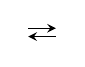
\begin{tikzpicture}[baseline]%
    \draw[>=stealth,<-](0,0.15ex)--(\arrlen,0.15ex);%
    \draw[>=stealth,->](0,0.85ex)--(\arrlen,0.85ex);%
  \end{tikzpicture}}}
\newcommand{\doubto}{\mathrel{%
  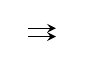
\begin{tikzpicture}[baseline]%
    \draw[>=stealth,->](0,0.15ex)--(\arrlen,0.15ex);%
    \draw[>=stealth,->](0,0.85ex)--(\arrlen,0.85ex);%
  \end{tikzpicture}}}
\newcommand{\lblto}[1]{\mathrel{%
    \begin{tikzpicture}[baseline= {( $ (current bounding box.south) + (0,-0.5ex) $ )}]
      \node[inner sep=.4ex] (a) {\,$\scriptstyle #1$\,};
      \draw[>=stealth,->] (a.south west) -- (a.south east);
    \end{tikzpicture}}}
\newcommand{\isoto}{\lblto{\sim}}

\newcommand{\simpl}[3]{
  \begin{tikzcd}[ampersand replacement=\&, column sep=small]
    #1 \&
    #2 \ar[l, shift right=0.35ex]
       \ar[l, shift left=0.35ex] \&
    #3 \ar[l, shift right=0.70ex]
       \ar[l, shift left=0.70ex]
       \ar[l] \&
    \cdots \ar[l, shift right=0.35ex]
           \ar[l, shift left=0.35ex]
           \ar[l, shift right=1.05ex]
           \ar[l, shift left=1.05ex]
  \end{tikzcd}
}
\newcommand{\cosimpl}[3]{
  \begin{tikzcd}[ampersand replacement=\&, column sep=small]
    #1 \ar[r, shift right=0.35ex]
       \ar[r, shift left=0.35ex] \&
    #2 \ar[r, shift right=0.70ex]
       \ar[r, shift left=0.70ex]
       \ar[r] \&
    #3 \ar[r, shift right=0.35ex]
       \ar[r, shift left=0.35ex]
       \ar[r, shift right=1.05ex]
       \ar[r, shift left=1.05ex] \&
    \cdots
  \end{tikzcd}
}

\newcommand{\tto}{\mathrel{\tikz[baseline]%
    \draw[>=stealth,->,double, double distance = 0.3ex](0,0.5ex)--(\arrlen,0.5ex);}}
\newcommand{\doubfrom}{\mathrel{%
  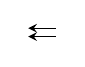
\begin{tikzpicture}[baseline]%
    \draw[>=stealth,<-](0,0.15ex)--(\arrlen,0.15ex);%
    \draw[>=stealth,<-](0,0.85ex)--(\arrlen,0.85ex);%
  \end{tikzpicture}}}
\newcommand{\tripfrom}{\mathrel{%
  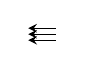
\begin{tikzpicture}[baseline]%
    \draw[>=stealth,<-](0,0.00ex)--(\arrlen,0.00ex);%
    \draw[>=stealth,<-](0,0.50ex)--(\arrlen,0.50ex);%
    \draw[>=stealth,<-](0,1.00ex)--(\arrlen,1.00ex);%
  \end{tikzpicture}}}


\renewcommand{\l}{\left}
\renewcommand{\r}{\right}
\newcommand{\f}{\frac}
\renewcommand{\o}{\overline}
\renewcommand{\u}{\underline}
\newcommand{\til}{\widetilde}
\renewcommand{\hat}{\widehat}
\newcommand{\del}{\partial}
\newcommand{\dash}{\text{-}}
\renewcommand{\c}{\colon}
\newcommand{\lc}{\,:\!}
\newcommand{\ce}{\coloneq}%{\mathrel{:=}}
\newcommand{\ec}{\eqcolon}%{\mathrel{=:}}
\newcommand{\iso}{\simeq}
\newcommand{\dual}{\vee}
\newcommand{\ldb}{\llbracket}
\newcommand{\rdb}{\rrbracket}

\newcommand{\Obj}{\operatorname{Obj}}
\newcommand{\Hom}{\operatorname{Hom}}
\newcommand{\Map}{\operatorname{Map}}
\newcommand{\Fun}{\operatorname{Fun}}
\newcommand{\Aut}{\operatorname{Aut}}
\newcommand{\Iso}{\operatorname{Iso}}
\renewcommand{\id}{\mathrm{id}}
\renewcommand{\im}{\operatorname{im}}
\newcommand{\op}{\mathrm{op}}
\newcommand{\univ}{\mathrm{univ}}
\newcommand{\colim}{\operatorname*{colim}}
\newcommand{\dlim}{\displaystyle\lim}
\newcommand{\dcolim}{\displaystyle\colim}
\newcommand{\Spec}{\operatorname{Spec}}
\newcommand{\Spf}{\operatorname{Spf}}

%%%%%%%%%%%%%%%%%%%%%%%%%%%%%%%%%%%%%%%%%%%%%%%%%%%%%%%%%%%%%%%%%%%%%%


\title{Math 216A Homework 1}
\author{Arpon Raksit}
\date{30 September 2016}

\numberwithin{block}{section}

%%%%%%%%%%%%%%%%%%%%%%%%%%%%%%%%%%%%%%%%%%%%%%%%%%%%%%%%%%%%%%%%%%%%%%


\begin{document}
\maketitle

\newcommand{\Alg}{\mathrm{Alg}}
\newcommand{\Set}{\mathrm{Set}}
\newcommand{\nil}{\mathrm{nil}}
\newcommand{\red}{\mathrm{red}}

%%%%%%%%%%%%%%%%%%%%%%%%%%%%%%%%%%%%%%%%%%%%%%%%%%%%%%%%%%%%%%%%%%%%%%

\section{Problem 1}

Let $R$ be a ring.

\begin{lemma}
  \label{fp-compact}
  Let $A$ be a finitely presented $R$-algebra. Then $A$ is a compact object of $\Alg_R$, i.e. the functor $\Map_{\Alg_R}(A,-) \c \Alg_R \to \Set$ preserves filtered colimits.
\end{lemma}

\begin{proof}
  Since $A$ is finitely presented we may write
  \[
    A \iso R[x_1,\ldots,x_n]/(f_1,\ldots,f_m)
      \iso \coeq(R[y_1,\ldots,y_m] \doubto R[x_1,\ldots,x_n]),
  \]
  where one of the maps $R[y_1,\ldots,y_m] \to R[x_1,\ldots,x_n]$ sends $y_i \mapsto f_i$ and the other sends $y_i \to 0$. It follows that we have a natural isomorphism
  \[
    \Map_{\Alg_R}(A,B) \iso \eq(B^n \doubto B^m),
  \]
  where one of the maps $B^n \to B^m$ sends $\u b = (b_1,\ldots,b_n) \mapsto (f_1(\u b), \ldots, f_m(\u b))$ and the other is the zero map. Now, filtered colimits in $\Alg_R$ are computed as filtered colimits in $\Set$, and in $\Set$ filtered colimits commute with finite limits (equivalently finite products and equalizers), so the above description of the functor $\Map_{\Alg_R}(A,-)$ shows that it 
preserves filtered colimits.
\end{proof}

\begin{proposition}
  \label{spread-map}
  Let $A,B$ be $R$-algebras. Suppose $A$ finitely presented. Let $\kp$ be a prime ideal in $A$ and $\kq$ a prime ideal in $B$. Let $F \c A_\kp \to B_\kq$ be a local $R$-algebra map. Then:
  \begin{enumerate}
  \item \label{spread-map-existence} There exist $b \in B \setminus \kq$ and an $R$-algebra map $f \c A \to B_b$ such that $f^{-1}(\kq_b) = \kp$ and $f_q = F$.
  \item \label{spread-map-uniqueness} For any two pairs $(b_1,f_1)$ and $(b_2,f_2)$ satisfying the conditions of \cref{spread-map-existence}, there exists $b \in B$ with $b_1,b_2 \mid b$ such that $f_1$ and $f_2$ become equal after composing with the canonical maps $B_{b_1} \to B_b$ and $B_{b_2} \to B$.
  \end{enumerate}
\end{proposition}

\begin{proof}
  First observe that, since $F$ is local, a pair $(b,f)$ satisfies the conditions of \cref{spread-map-existence} if and only if the diagram
  \[
    \begin{tikzcd}
      A \ar[r, "f"] \ar[d, "\phi", swap] &
      B_b \ar[d, "\psi"] \\
      A_\kp \ar[r,"F"] &
      B_\kq
    \end{tikzcd}
  \]
  commutes. Then recall that we have $B_\kq \iso \colim_{b \in B \setminus \kq} B_b$, where the colimit is over the directed set $B \setminus \kq$ (ordered by divisibility). Since $A$ is finitely presented, \cref{fp-compact} implies that the canonical map
  \[
    \colim_{b \in B \setminus \kq} \Map_{\Alg_R}(A, B_b) \to \Map_{\Alg_R}(A, B_\kq)
  \]
  is a bijection. Considering the element $F \circ \phi \c A \to B_\kq$ on the right-hand side, surjectivity gives us \cref{spread-map-existence} and injectivity gives us \cref{spread-map-uniqueness}.
\end{proof}

%%%%%%%%%%%%%%%%%%%%%%%%%%%%%%%%%%%%%%%%%%%%%%%%%%%%%%%%%%%%%%%%%%%%%%

\section{Problem 2}

Let $k$ be an algebraically closed field.

\begin{lemma}
  \label{reduced-tensor}
  Let $A,B$ be $k$-algebras. Suppose $B$ is reduced. If $A$ is reduced or a domain then $B \otimes_k A$ is the same.
\end{lemma}

\begin{proof}
  Since subrings and filtered colimits of reduced rings or domains are the same, and tensor product commutes with colimits, writing $B$ as the filtered colimit of its subalgebras allows us to restrict to the case that $B$ is of finite type. We then have that $\bigcap_{\km \in \Specm B} \km$ is the nilradical of $B$ \footnote{This comes down to the following fact: if $C \to D$ is a map of $k$-algebras (here $k$ can be any field) and $D$ is of finite type over $k$, then the preimage of a maximal ideal is not just prime but maximal.}, which is $0$ since $B$ is reduced. Thus the canonical map
  \[
    B \to \prod_{\km \in \Specm B} B/\km
  \]
  is an injection. Since everything is flat over a field, this gives us an injection
  \[
    B \otimes_k A \inj \l(\prod_{\km \in \Specm B} B/\km\r) \otimes_k A.
  \]
  By the Nullstellensatz each $B/\km$ is isomorphic to $k$, whence the right-hand side above is isomorphic to $A^I$, $I$ being the set $\Specm B$. If $A$ is reduced or a domain then so is $A^I$, and hence so must be $B \otimes_k A$.
\end{proof}

\begin{remark}
  \label{reduced-tensor-fail}
  Note that \cref{reduced-tensor} can fail when $k$ is not algebraically closed. E.g. if $L$ is a nontrivial finite $G$-Galois extension of $k$ then $L \otimes_k L \iso L^G$ is not a domain; and if we take $k$ to be non-perfect and $L$ a nontrivial purely inseperable extension of $k$ then $L \otimes_k L$ will not even be reduced.
\end{remark}

\begin{proposition}
  \label{field-extension-prop-1}
  Let $k'$ be an extension field of $k$. Let $A$ be a $k$-algebra, and $A' \ce k' \otimes_k A$. Let $\rP$ be one of the following properties of rings:
  \begin{enumerate}
  \item \label{field-extension-prop-non-zero} is non-zero;
  \item \label{field-extension-prop-reduced} is reduced;
  \item \label{field-extension-prop-domain} is a domain;
  \end{enumerate}
  then $A$ satisfies $\rP$ if and only if $A'$ satisfies $\rP$.
\end{proposition}

\begin{proof}
  \begin{enumerate}[leftmargin=*]
  \item If $A$ is zero, clearly $A'$ is zero. If $A$ is non-zero, then since everything is flat over a field, the injection $k \inj k'$ induces an injection $A \inj A'$, so $A'$ is also non-zero.

  \item If $A$ is reduced then by \cref{reduced-tensor} so is $A'$. The converse again follows from the injection $A \inj A'$.

  \item Same as \cref{field-extension-prop-reduced}. \qedhere
  \end{enumerate}
\end{proof}

\begin{lemma}
  \label{field-extension-ideal}
  Let $k'$ be an extension field of $k$. Let $A$ be a $k$-algebra, and $A' \ce k' \otimes_k A$. Let $\kp$ be a prime ideal in $A$, and $\kp' \ce k' \otimes_k \kp$. Then:
  \begin{enumerate}
  \item \label{field-extension-ideal-prime} $\kp'$ is a prime ideal in $A'$;
  \item \label{field-extension-ideal-maximal} if we assume moreover that $A$ is of finite type and $\kp$ is maximal, then $\kp'$ is maximal.
  \end{enumerate}
\end{lemma}

\begin{proof}
  By flatness over a field, the exact sequence $0 \to \kp \to A \to A/\kp \to 0$ induces an exact sequence $0 \to \kp' \to A' \to k' \otimes_k A/\kp \to 0$, implying that $\kp'$ indeed includes into $A'$ as an ideal, and that $A'/\kp' \iso k' \otimes_k A/\kp$. Then:
  \begin{enumerate}
  \item By \cref{field-extension-prop-1}\cref{field-extension-prop-domain}, $A/\kp$ being a domain implies $A'/\kp'$ is a domain, so $\kp'$ is prime.
  \item If $A$ is of finite type and $\kp$ is maximal, then by the Nullstellensatz $A/\kp \iso k$, so $A'/\kp' \iso k'$ is a field, so $\kp'$ is also maximal. \qedhere
  \end{enumerate}
\end{proof}

\begin{proposition}
  \label{field-extension-prop-2}
  Let $k'$ be an extension field of $k$. Let $A$ be a $k$-algebra, and $A' \ce k' \otimes_k A$. Let $\rP$ be one of the following properties of rings:
  \begin{enumerate}
  \item \label{field-extension-prop-irreducible} has a unique minimal prime;
  \item \label{field-extension-prop-dimension} is of dimension $d$;
  \end{enumerate}
  then $A$ satisfies $\rP$ if and only if $A'$ satisfies $\rP$.
\end{proposition}

\begin{proof}
  \begin{enumerate}[leftmargin=*]
  \item A ring has a unique minimal prime (i.e. its spectrum is irreducible) if and only if its nilradical is a prime ideal. Consider the exact sequences
    \[
      0 \to A^\nil \to A \to A^\red \to 0, \quad
      0 \to (A')^\nil \to A' \to (A')^\red \to 0.
    \]
    It suffices to show that $A^\red$ is a domain if and only if $(A')^\red$ is a domain. The ``if'' direction follows from the fact that the injection $A \inj A'$ induces an injection $A^\red \inj (A')^\red$. Let's prove ``only if''. By \cref{field-extension-ideal-prime}, if $A^\red$ is a domain, so is $k' \otimes_k A^\red$. But then in particular it is reduced, so we must have $(A')^\nil = k' \otimes_k A^\nil$, which finishes.

  \item We will prove that $\dim A = \dim A'$. We have
    \[
      \dim A = \sup \dim A/\kp, \quad
      \dim A' = \sup \dim A'/\kp',
    \]
    where the suprema are taken over the minimal primes in each ring. Given a prime $\kp'$ of $A'$, if we let $\kp$ be its preimage in $A$, then by \cref{field-extension-ideal}\cref{field-extension-ideal-prime} $k' \otimes_k \kp$ is a prime in $A'$, evidently contained in $\kp'$. Thus all minimal primes of $A'$ must be of the form $k' \otimes_k \kp$. It therefore suffices to show that for a (minimal) prime $\kp$ of $A$, $\dim A/\kp = \dim A'/\kp'$ for $\kp' \ce k' \otimes_k \kp$. Using flatness to obtain the exact sequence
    \[
      0 \to k' \otimes_k \kp \to A' \to k' \otimes_k (A/\kp) \to 0,
    \]
    we identify $A'/\kp'$ with $k' \otimes_k (A/\kp)$ and are thus reduced to the case that $A$ is a domain. Then by Noether normalization there exists a finite map of $k$-algebras $k[t_1,\ldots,t_d] \to A$ for $d = \dim A$. Base-changing gives us a finite map of $k'$-algebras $k'[t_1,\ldots,t_d] \to A'$. By \cref{field-extension-prop-1}\cref{field-extension-prop-domain} $A'$ is also a domain, so we must also have $d = \dim A'$. \qedhere
  \end{enumerate}
\end{proof}

\begin{proposition}
  \label{field-extension-prop-regular}
  Let $k'$ be an algebraically closed extension field of $k$. Let $A$ be a $k$-algebra of finite type, and $A' \ce k' \otimes_k A$. Then $A$ is regular if and only if $A'$ is regular.
\end{proposition}

\begin{proof}
  We use the Jacobian criterion: by \cref{field-extension-prop-2}\cref{field-extension-prop-dimension} $\dim A = \dim A'$, and the corank of the Jacobian of a presentation $A \iso k[t_1,\ldots,t_n]/(f_1,\ldots,f_m)$ is independent of whether we compute it over $k$ or $k'$.
\end{proof}

%%%%%%%%%%%%%%%%%%%%%%%%%%%%%%%%%%%%%%%%%%%%%%%%%%%%%%%%%%%%%%%%%%%%%%

\section{Problem 3}

\begin{proposition}
  \label{irreducibility-reformulation}
  Let $R$ be a ring and $f \in R[t_1,\ldots,t_n]$ a polynomial. There is a collection of polynomials $\chi_1(f),\ldots,\chi_r(f) \in R[a_1,\ldots,a_s]$ satisfying the following:
  \begin{enumerate}
  \item \label{irreducibility-reformulation-base} $f$ is irreducible over $R$ if and only if $\chi_1(f),\ldots,\chi_r(f)$ admit no common solution over $R$;
  \item \label{irreducibility-reformulation-functor} the values $r$ and $s$ depend only on the degree of $f$, and $\chi_1(f),\ldots,\chi_r(f)$ are functorial in the pair $(R,f)$, in the sense that if $\phi \c R \to S$ is a ring map under which the polynomial $f$ is sent to $g \in S[t_1,\ldots,t_n]$, then $\phi$ sends $\chi_i(f)$ to $\chi_i(g)$ for $1 \le i \le r$.
  \item \label{irreducibility-reformulation-geometric} for any $R$-algebra $K$ which is a field, and any algebraically closed field $K'$ containing $K$, $f$ is irreducible over $K'$ if and only $\chi_1(f),\ldots,\chi_r(f)$ generate the unit ideal in $K[a_1,\ldots,a_s]$.
  \end{enumerate}
\end{proposition}

\begin{proof}
  \begin{enumerate}[leftmargin=*]
  \item Write out the condition you get on the coefficients for two polynomials of degree lower than $f$ to multiply to $f$.
  \item Evident from the construction of \cref{irreducibility-reformulation-base}.
  \item Apply \cref{irreducibility-reformulation-base} over $K'$ and then the Nullstellensatz over $K$. \qedhere
  \end{enumerate}
\end{proof}

\begin{remark}
  Note that \cref{irreducibility-reformulation}\cref{irreducibility-reformulation-geometric} implies that if $f$ is irreducible over an algebraically closed field containing $K$, it is irreducible over all algebraically closed fields containing $K$.
\end{remark}

\begin{proposition}
  \label{char-0-to-char-p}
  Let $f \in \lZ[t_1,\ldots,t_n]$ be an integer polynomial which is irreducible over $\o \lQ$. Then for all but finitely many primes $p$, the reduction $\til f \in \lF_p[t_1,\ldots,t_n]$ modulo $p$ is irreducible over $\o{\lF_p}$.
\end{proposition}

\begin{proof}
  Let $\chi_1(f),\ldots,\chi_r(f) \in \lZ[a_1,\ldots,a_s]$ be the polynomials supplied by \cref{irreducibility-reformulation}. Applying \cref{irreducibility-reformulation}\cref{irreducibility-reformulation-geometric},  we obtain $\alpha_1,\ldots,\alpha_r \in \lQ[a_1,\ldots,a_s]$ such that $\sum \alpha_i\chi_i(f) = 1$. Clearing denominators gives us $\beta_1,\ldots,\beta_r \in \lZ[a_1,\ldots,a_s]$ such that $\sum \beta_i\chi_i(f) = N$ for some $N \in \lZ$. Then for any prime $p$ not dividing $N$, using the functoriality guaranteed by \cref{irreducibility-reformulation}\cref{irreducibility-reformulation-functor}, we get
  \[
    \frac{1}{N} \sum_i \til\beta_i \chi_i(\til f) = 1 \in \lF_p[t_1,\ldots,t_n],
  \]
  and we finish by once more applying \cref{irreducibility-reformulation}\cref{irreducibility-reformulation-geometric}.
\end{proof}

%%%%%%%%%%%%%%%%%%%%%%%%%%%%%%%%%%%%%%%%%%%%%%%%%%%%%%%%%%%%%%%%%%%%%%

\section{Problem 4}

\begin{proposition}
  Let $(A,\km)$ be a complete local noetherian ring. Suppose there is a subfield $k \subseteq A$ such that the map $k \to A/\km$ is an isomorphism. Then $A$ is regular if and only if there is an isomorphism of $k$-algebras $A \iso k\llbracket t_1,\ldots,t_n \rrbracket$.
\end{proposition}

\begin{proof}
  The ``if'' direction is clear, since we know $R \ce k\llbracket t_1,\ldots,t_n \rrbracket$ is regular. So let's prove ``only if''. Assume $A$ is regular, so we can pick a generating set $x_1,\ldots,x_n$ of $\km$ with $n \ce \dim A$. By the universal property of $R$, there's a unique $k$-algebra map $\phi \c R \to A$ sending $t_i \mapsto x_i$ for $1 \le i \le n$.

  We first show that $\phi$ must be surjective. Let $a \in A$. We inductively construct a sequence $f_0,f_1,\ldots$ in $R$ such that:
  \begin{itemize}
  \item $f_i$ is a homogenous polynomial of degree $i$
  \item $\phi(\sum_{j=0}^i f_j) - a \in \km^i$
  \end{itemize}
  Then $f \ce \sum_i f_i$ will be a well-defined element of $R$ and by continuity we will have $\phi(f) - a \in \bigcap \km^i = 0$, hence $\phi(f) = a$.
  For the base case, we may choose $f_0 = 0$ (we're taking $\km^0 = (1) = A$ by convention). Suppose we have constructed $f_i$. Since $(x_1,\ldots,x_n)$ generate $\km$, we may write (using multi-index notation)
  \[
    \phi(f_i) - a = \sum_{\u I} a_{\u I} \u x^{\u I},
  \]
  where $\u I$ runs over tuples in $\lZ_{\ge 0}^n$ which sum to $i$. Since $k \to A/\km$ is an isomorphism, we may choose $c_{\u I} \in k$ such that $\phi(c_{\u I}) - a_{\u I} \in \km$. Then we set
  \[
    f_{i+1} = \sum_{\u I} c_{\u I} \u t^{\u I},
  \]
  and it's easy to see this satisfies the required properties.

  So we've proven $\phi$ is surjective, and we now show it's in fact an isomorphism. Let $\kp \ce \ker(\phi)$, which is prime since $A$ is a domain. Then $\phi$ induces an isomorphism $R/\kp \to A$, so $\dim R/\kp = n$. But this can only happen if $\kp = 0$, so we're done.
\end{proof}

\begin{proposition}
  \label{nonperfect-weird}
  Let $K$ be a field of characteristic $p$. Suppose $a \in K$ is not a $p$-th power, so $K$ is not perfect and $t^p - a \in K[t]$ is irreducible. Let $\kp \ce (t^p - a) \in \Spec K[t]$. Let $A \ce \hat{K[t]_\kp}$. Then:
  \begin{enumerate}
  \item \label{nonperfect-weird-normalness} $A$ is a complete DVR with residue field isomorphic to $K(a^{1/p})$ (as $K$-algebras).
  \item \label{nonperfect-weird-weirdness} There is no subfield $k \subseteq A$ containing $K$ such that the map $k \to A/\km$ is an isomorphism.
  \end{enumerate}
\end{proposition}

\begin{proof}
  \begin{enumerate}[leftmargin=*]
  \item $K[t]$ is a regular ring of dimension $1$ and $\kp$ is maximal, so $K[t]_\kp$ is a DVR, with residue field isomorphic to $K[t]/\kp \iso K(a^{1/p})$. The same is then true of its completion, $A$.

  \item Suppose there were such a subfield $k$. Then (by flatness over a field) we would obtain an inclusion $k \otimes_K k \to k \otimes_K A$, and
    \[
      k \otimes_K k \iso K(a^{1/p})[t]/(t^p-a) \iso K(a^{1/p})[t]/(t-a^{1/p})^p
    \]
    is non-reduced. We claim however that $k \otimes_K A$ is reduced, giving us a contradiction. Indeed, we have
    \begin{align*}
      k \otimes_K A &\iso k \otimes_K K[t]_\kp \otimes_{K[t]_\kp} \hat{K[t]_\kp} \\
                    &\iso k[t]_{\kp'} \otimes_{K[t]_\kp} \hat{K[t]_\kp} \\
                    &\iso \hat{k[t]_{\kp'}},
    \end{align*}
    where $\kp' = (t - a^{1/p}) \in \Spec k[t]$ \footnote{Here we've used that localizing/completing with respect to $\kp = (\kp')^p$ is the same as localizing/completing with respect to $\kp'$, and that completing a module or algebra over a noetherian base ring is equivalent to tensoring with the completion of the base.}, so $k \otimes_k A$ is also a DVR, hence reduced. \qedhere
  \end{enumerate}
\end{proof}

\begin{remark}
  \label{cohen-uncontradicted}
  Let $A$ be as in \cref{nonperfect-weird}. The Cohen structure theorem implies that there is an isomorphim $A \iso K(a^{1/p})\llbracket t \rrbracket$. This does not contradict \cref{nonperfect-weird}\cref{nonperfect-weird-weirdness} because the Cohen structure theorem doesn't tell us that the isomorphism must be one of $K$-algebras. Hence there is a copy of $K(a^{1/p})$ inside $A$, but it can't contain $K$ as a subfield!
\end{remark}

%%%%%%%%%%%%%%%%%%%%%%%%%%%%%%%%%%%%%%%%%%%%%%%%%%%%%%%%%%%%%%%%%%%%%%

\end{document}
